% !TeX root = 系统动力学建模与仿真笔记.tex
众所周知，艾萨克·牛顿和戈特弗里德·莱布尼茨各自独立地发明了微积分。不太为人所知的是，他们对质点系统的时间演化有不同的看法。牛顿第二定律给出了作用在质点上的力与其加速度之间的矢量关系。（对于由 $N$ 个质点组成的系统，我们有 $N$ 个矢量关系，对应 $3N$ 个标量二阶微分方程。这些方程通常是耦合的，因为所有 $N$ 个质点的位置都可能出现在 $3N$ 个运动方程中的每一个里面。要确定运动，我们必须同时求解所有这些耦合方程。）

另一方面，莱布尼茨认为，通过考察质点的"活力"（vis-viva），或者用我们今天的话说，它们的动能，可以更好地分析质点的运动。

从根本上说，牛顿认为量 $m_iv_i$ 在运动过程中是守恒的，而莱布尼茨认为 $m_iv_i^2$ 是常数。用现代术语来说，牛顿相信动量守恒，而莱布尼茨相信动能守恒。不久就清楚了，动能（$T$）在系统运动过程中并不守恒，但当势能（$V$）的概念引入后，莱布尼茨的理论被扩展为：总能量（$E = T + V$）是常数，这当然是力学的基本守恒定律之一。因此，你可以说，牛顿和莱布尼茨都是正确的。

在初级物理课程中，我们经常在牛顿定律和能量守恒之间切换使用。例如，落体问题可以用 $F = ma$ 求解，也可以用能量守恒求解。

后来，欧拉和拉格朗日发展了莱布尼茨的思想，并表明系统的运动可以由一个统一的原理来预言，我们现在称之为哈密顿原理。有意思的是，这种方法不涉及矢量，甚至不涉及力，尽管力可以从它导出。欧拉和拉格朗日的方法称为"分析力学"。

分析力学不要求牛顿三大定律，尤其不需要第三定律。有些物理学家认为，牛顿引入第三定律是为了处理约束问题。（弹跳的球被"约束"在房间内。在牛顿的图像中，球从墙上弹回，是因为墙对它施加了一个反作用力，正如第三定律所给出的那样。）拉格朗日方法把约束纳入分析的框架，第二定律和第三定律都不是必需的。然而，约束力和运动方程都可以由该方法确定。此外，分析力学中的所有方程都是标量方程，所以我们不需要使用矢量分析的任何概念。来看看吧！
\section{广义坐标}
在高中的时候我们描述一个平面里的运动，一般有两种形式，一种是$x$-$y$坐标系下的运动，另一种是极坐标系$r$-$\theta$下的运动。无论怎么描述，都需要两个独立的坐标。
而在空间中我们描述一个物体的运动，可以使用$x$$y$$z$三个坐标。当然也可以使用$r$-$\theta$-$\phi$三个坐标。无论怎么描述，都需要三个独立的坐标。进一步地，在三维空间中确定单个质点的位置需要三个坐标，对于由 $N$ 个质点组成的系统则需要 $3N$ 个坐标；在笛卡尔坐标中，$N$ 个质点的位置可由数集 $(x_1, y_1, z_1, x_2, y_2, z_2, \cdots, x_N, y_N, z_N)$ 描述。

由此，我们不禁思考坐标是什么。于是有广义坐标：

\begin{mydefinition}{广义坐标}
广义坐标是用来描述系统位形所需要的独立参数，或者最少参数的集合。广义坐标的个数就是系统的自由度。
\end{mydefinition}
下面我们需要思考广义坐标和Cartesian坐标之间的关系。我们知道，广义坐标是最少参数的集合，而Cartesian坐标是描述系统位形所需要的参数集合。
因为描述的是同一个系统，所以广义坐标和Cartesian坐标之间是有关系的。我们可以用一个函数来描述这种关系：
\begin{equation}\label{eq:1.1}
\bm{q} = \bm{q}(\bm{x},t)
\end{equation}
展开来看就是：
    \begin{equation}\label{eq:1.2}
\begin{bmatrix} q_1 \\ q_2 \\ \vdots \\ q_n \end{bmatrix} = \begin{bmatrix} q_1(x_1,x_2,\cdots,x_n,t) \\ q_2(x_1,x_2,\cdots,x_n,t) \\ \vdots \\ q_n(x_1,x_2,\cdots,x_n,t) \end{bmatrix}
\end{equation}
那么就有逆关系，也称为\textbf{变换方程(transformations equation)}：
\begin{equation}\label{eq:1.3}
\bm{x} = \bm{x}(\bm{q},t)
\end{equation}
展开来看就是：
\begin{equation}\label{eq:1.4}
\begin{bmatrix} x_1 \\ x_2 \\ \vdots \\ x_n \end{bmatrix} = \begin{bmatrix} x_1(q_1,q_2,\cdots,q_n,t) \\ x_2(q_1,q_2,\cdots,q_n,t) \\ \vdots \\ x_n(q_1,q_2,\cdots,q_n,t) \end{bmatrix}
\end{equation}
式中，$\bm{q}$是广义坐标，$\bm{x}$是Cartesian坐标。

但变换方程不一定存在，需满足Jacobian矩阵的条件。
\begin{equation}\label{eq:1.5}
\det\left(\frac{\partial(q_1, q_2, \cdots, q_n)}{\partial(x_1, x_2, \cdots, x_n)}\right) \neq 0.
\end{equation}

通常假定广义坐标是线性无关的，因而构成描述系统位形的极小坐标集。例如，半径为 $a$ 的球面上的质点，其位置可以用两个角（如经度和纬度）来描述，这两个角构成一个由线性无关坐标组成的极小集。然而，我们也可以用三个笛卡尔坐标 $x$、$y$、$z$ 来描述质点的位置，但显然这不是一个极小集，原因是笛卡尔坐标并非全部独立，它们满足关系 $x^2 + y^2 + z^2 = a^2$。注意，给定 $x$ 和 $y$，坐标 $z$ 就确定了。这样的关系称为\textbf{约束（constraint）}。每一条约束方程都把独立坐标的数目减少一个。

还需指出，虽然笛卡尔坐标具有矢量的分量这一性质，但广义坐标未必如此。在球面上质点的例子中，两个角是一组合适的广义坐标，但它们并不是矢量的分量。事实上，广义坐标甚至不必是通常意义下的坐标。

\section{位形空间（Configuration Space）}
什么是位形？此前在 Lynch 的《现代机器人学》中也出现过这一概念。

书上的定义是：确定系统中所有质点的位置，称为系统的位形。一般说来，由 $N$ 个自由质点组成的系统的位形由下式给出
\begin{equation}\label{eq:cs}
(q_1, q_2, \ldots, q_n), \qquad \text{其中 } n = 3N.
\end{equation}
可以看到，由 $N$ 个质点组成的系统的位形，用 $3N$ 维参考系中的一个点表示。

考虑单个质点的三维参考系。随着时间推移，坐标的值发生变化。这种变化是连续的，表示质点位置的点将描绘出一条光滑曲线。类似地，在以广义坐标为轴、维数为 $n$ 的位形空间中，表示系统位形的点将描绘出一条光滑曲线，它表示系统的时间演化。

值得指出，当我们从一组坐标变换到另一组坐标时，位形空间的特征可能发生显著变化。直线可能变成曲线，角和距离可能改变。然而，某些几何性质保持不变。点仍然是点，曲线仍然是曲线。相邻的曲线保持相邻，一个点的邻域保持为该点的邻域（虽然邻域的形状可能会不同）。

\begin{remark}
为什么（从数学的角度能解释吗？）：坐标变换是位形空间上的微分同胚，光滑曲线、相邻关系与开邻域在微分同胚下保持不变，而直线、角和距离取决于具体的度量结构，会随坐标选择而改变。
\end{remark}

\section{相空间（Phase Space）}
用质点的位置和动量来描述质点系统往往很方便。系统的"状态"用某一时刻所有质点的位置和动量的值来描述。例如，我们可以用笛卡尔坐标 $x_i$、$i = 1, 2, 3$ 来表示质点的位置。类似地，质点的动量可以用 $p_i$、$i = 1, 2, 3$ 表示。想象画一个 $2n$ 维坐标系，其轴标为 $x_1, \ldots, x_n$；$p_1, \ldots, p_n$。由这组轴所描述的空间称为相空间。所有质点的位置以及所有质点的动量，由相空间中的单个点来表示。随着时间推进，每个质点的位置和动量都发生变化。这些变化是连续的，所以相空间中的点在 $2n$ 维坐标系中连续运动。也就是说，系统的时间演化可以用相空间中的一条轨迹来表示。这条轨迹称为\textbf{相路径}，在某些文献中也称为\textbf{世界线}。

\section{约束}

一般说来，由 $N$ 个自由质点组成的力学系统有 $3N$ 个自由度。约束的作用是减少描述运动所需的坐标数目，即减少独立坐标个数；一个约束减少系统的一个自由度。如果由 $N$ 个质点组成的系统受到 $k$ 个约束的作用，那么描述运动所需的广义坐标数目为 $3N - k$。

由此可知约束本质上是坐标之间的关系。存在约束的坐标之间不相互独立。换句话说，相互独立的坐标间不存在约束。

\begin{mydefinition}{完整约束}
如果约束方程可以表示成
$$f(q_1, q_2, \ldots, q_n, t) = 0$$
的形式，则这个约束称为\textbf{完整约束（holonomic constraint）}。
\end{mydefinition}

比如被约束在球面上的质点：其坐标满足关系 $x^2 + y^2 + z^2 - a^2 = 0$，这就是一个完整约束。完整约束定义的关键要素是：\textcircled{1} 等号；\textcircled{2} 它是涉及坐标的关系。例如，质点总是处于半径为 $a$ 的球的外部，即 $r \geq a$，这不是完整约束。有时约束不仅涉及坐标，还涉及速度或坐标的微分，这样的约束也不是完整的。

作为非完整约束的一个例子，考虑一个在完全粗糙的桌面上滚动的弹珠。弹珠需要五个坐标来完整描述它的位置和取向：两个线坐标给出它在桌面上的位置，三个角坐标描述它的取向。如果桌面是完全光滑的，弹珠可以滑动，线坐标与角坐标之间就没有关系。但如果桌面是粗糙的，角坐标与线坐标之间就有关系（约束），这些约束具有一般形式 $dr = a\,d\theta$，这是微分之间的关系。如果这样的微分表达式可以积分，那么约束就变成坐标之间的关系，它就是完整的。但一般说来，在平面上的滚动并不导致可积分的关系，即滚动约束不是完整的。但沿直线的滚动是可积的，因而是完整的。

\begin{mydefinition}{定常约束}
不显含时间的约束称为\textbf{定常约束（scleronomous constraint）}。
\end{mydefinition}

使用广义坐标和传统坐标的一个区别在于：使用广义坐标的时候，约束越多，广义坐标数目反而越少。完整约束联系广义坐标的方程，可以用来用一个坐标表示其他坐标，从而减少描述运动所需的坐标数目。

\begin{example}[珠子在运动导线上滑动]
一颗珠子在一根以复杂方式在空间中运动的导线上滑动。这个约束是完整的吗？它是定常的吗？
\end{example}

\begin{solution}
珠子被限制在导线上，意味着珠子在任何时刻都必须位于导线的几何位置上。设导线的空间曲线方程在时刻 $t$ 可以表示为 $F(x, y, z, t) = 0$，则约束方程即为 $F(x, y, z, t) = 0$。该方程只涉及坐标和时间，不包含速度，因此它是\textbf{完整约束}。广义坐标可简化为沿导线的弧长 $s$，不改变其完整性的本质。

判断约束是否定常，核心标准是约束方程中是否显含时间 $t$。题目指出导线以复杂方式在空间中运动，意味着导线的空间曲线方程随时间改变，$\dfrac{\partial F}{\partial t}\neq 0$，因此该约束是\textbf{非定常约束（rheonomic constraint）}。
\end{solution}

\begin{example}[双原子分子的自由度]
考虑一个双原子分子。假设原子是质点。分子可以转动，也可以沿连接两原子的直线振动。它有几个转动轴？分子有多少个自由度？
\end{example}

\begin{solution}
连接两原子的直线称为分子轴。绕分子轴旋转时，两个质点的空间位置没有任何变化，终态与初态无法区分，因此不算有效的转动轴。垂直于分子轴的轴方向有无数条，但它们在物理上线性相关，只需 2 个独立的角度（如极角 $\theta$ 和方位角 $\phi$）就能描述所有转动状态，故有 \textbf{2 个转动轴}。

对于 $N=2$ 的质点系统，总机械自由度为 $3\times2=6$，分解为：
\begin{itemize}
    \item \textbf{平动自由度（3 个）}：分子整体在三维空间中的质心平动（$X, Y, Z$）
    \item \textbf{转动自由度（2 个）}：描述分子轴在空间中的朝向（$\theta, \phi$）
    \item \textbf{振动自由度（1 个）}：沿分子轴方向，原子间相对距离的变化（键长 $r$ 的伸缩）
\end{itemize}
共 \textbf{6 个自由度}。
\end{solution}
\section{广义速度}
坐标有广义坐标，速度自然有广义速度。
\begin{mydefinition}{广义速度}
广义速度是广义坐标的导数。即$$\dot{\bm{q}} = \frac{d\bm{q}}{dt}$$
\end{mydefinition}

广义坐标与笛卡尔坐标通过变换方程~(\ref{eq:1.3})~彼此联系。对于某个笛卡尔坐标分量 $x_i = x_i(q_1, q_2, \cdots, q_n, t)$，它（一般）依赖于所有的广义坐标。利用微分的链式法则，笛卡尔速度分量 $v_i$ 可表示为
\begin{equation}\label{eq:1.6}
v_i \equiv \frac{dx_i}{dt} = \sum_{k=1}^{n}\frac{\partial x_i}{\partial q_k}\frac{dq_k}{dt} + \frac{\partial x_i}{\partial t} = \sum_{k=1}^{n}\frac{\partial x_i}{\partial q_k}\dot{q}_k + \frac{\partial x_i}{\partial t}.
\end{equation}

由上式可以导出一个在后续推导中非常常用的关系式。
\begin{proof}[推导]
由于 $x_i$ 不依赖于广义速度 $\dot{q}$，即 $\dfrac{\partial x_i}{\partial \dot{q}_j} = 0$，利用式~(\ref{eq:1.6})~求 $v_i$ 对 $\dot{q}_j$ 的偏导数，可得
\begin{equation}\label{eq:1.7}
\frac{\partial v_i}{\partial \dot{q}_j} = \frac{\partial}{\partial \dot{q}_j}\sum_{k=1}^{n}\frac{\partial x_i}{\partial q_k}\dot{q}_k = \sum_{k=1}^{n}\frac{\partial x_i}{\partial q_k}\frac{\partial \dot{q}_k}{\partial \dot{q}_j} = \sum_{k=1}^{n}\frac{\partial x_i}{\partial q_k}\delta_{kj} = \frac{\partial x_i}{\partial q_j}.
\end{equation}
于是，我们得出结论
\begin{equation}\label{eq:1.8}
\frac{\partial v_i}{\partial \dot{q}_j} = \frac{\partial x_i}{\partial q_j}.
\end{equation}
\end{proof}
这个简单的关系式在许多涉及广义坐标的推导中非常有用，它说明：笛卡尔速度与广义速度的关系，与笛卡尔坐标与广义坐标的关系相同。

\section{虚位移}
虚位移 $\delta x$ 定义为坐标 $x$ 的无穷小瞬时位移，且与作用在系统上的任何约束相容。
为了理解普通位移 $dx_i$ 与虚位移 $\delta x$ 之间的差别，考虑变换方程$$x = x(q_1, q_2, \ldots, q_n, t), \qquad i = 1, 2, \ldots, 3N.$$
对变换方程取微分，我们得到$$dx_i = \frac{\partial x}{\partial q_1}dq_1 + \frac{\partial x}{\partial q_2}dq_2 + \cdots + \frac{\partial x}{\partial q_n}dq_n + \frac{\partial x}{\partial t}dt = \sum_{\alpha=1}^{n}\frac{\partial x}{\partial q_\alpha}dq_\alpha + \frac{\partial x}{\partial t}dt.$$
但对于虚位移 $\delta x$，时间是冻结的即$\frac{\partial x}{\partial t}dt=0$，所以$$\delta x = \sum_{\alpha=1}^{n}\frac{\partial x}{\partial q_\alpha}\delta q_\alpha. $$

\section{虚功和广义力}

假设一个系统受到若干主动力的作用。设 $F_i$ 是沿 $x$ 方向的力分量。（于是，对两质点系统，$F_5$ 将是作用在质点 2 上沿 $y$ 方向的力。）让所有笛卡尔坐标经历虚位移 $\delta x$，则主动力所做的虚功为
\begin{equation}\label{eq:1.vw}
\delta W = \sum_{i=1}^{3N}F_i\,\delta x_i.
\end{equation}
把式~(\ref{eq:1.vw})~中的 $\delta x_i$ 利用虚位移的表达式代入，得到
\begin{equation*}
\delta W = \sum_{i=1}^{3N}F_i\sum_{\alpha=1}^{3N}\frac{\partial x_i}{\partial q_\alpha}\delta q_\alpha.
\end{equation*}
交换求和次序，
\begin{equation*}
\delta W = \sum_{\alpha=1}^{3N}\left(\sum_{i=1}^{3N}F_i\frac{\partial x_i}{\partial q_\alpha}\right)\delta q_\alpha.
\end{equation*}
而我们的印象里，功应该等于力乘位移，于是引入广义力：

\begin{mydefinition}{广义力}
广义力定义为
\begin{equation}\label{eq:1.gf}
Q_\alpha = \sum_{i=1}^{3N}F_i\frac{\partial x_i}{\partial q_\alpha}.
\end{equation}
\end{mydefinition}

\begin{example}[虚功原理蕴含合力矩为零]
证明虚功原理（平衡时 $\delta W = 0$）蕴含着作用在物体上的力矩之和必须为零。
\end{example}

\begin{solution}
选一个沿任意方向的转轴。设物体绕该轴转过一个无穷小角度 $\epsilon$。位于 $\mathbf{R}_i$ 处的点 $P_i$ 相对于轴的虚位移由下式给出
\begin{equation*}
\delta\mathbf{R}_i = \bm{\epsilon}\times\mathbf{R}_i.
\end{equation*}
作用在 $P_i$ 上的力 $\mathbf{F}_i$ 所做的虚功为
\begin{equation*}
\delta W_i = \mathbf{F}_i\cdot\delta\mathbf{R}_i = \mathbf{F}_i\cdot(\bm{\epsilon}\times\mathbf{R}_i) = \bm{\epsilon}\cdot(\mathbf{R}_i\times\mathbf{F}_i) = \bm{\epsilon}\cdot\mathbf{N}_i,
\end{equation*}
其中 $\mathbf{N}_i$ 是绕轴作用在 $P_i$ 上的力矩。总的虚功为
\begin{equation*}
\delta W = \sum_i \bm{\epsilon}\cdot\mathbf{N}_i = \bm{\epsilon}\cdot\sum_i\mathbf{N}_i = \bm{\epsilon}\cdot\mathbf{N}_{\mathrm{tot}}.
\end{equation*}
对不转动的物体，$\bm{\epsilon}$ 的方向是任意的，所以由虚功原理 $\delta W = 0$ 可得 $\mathbf{N}_{\mathrm{tot}} = 0$，即作用在物体上的力矩之和必须为零。
\end{solution}

\section{求运动方程}
由牛顿三大定律给出的运动方程通常具有如下形式
\begin{equation}\label{eq:1.eom}
\ddot{x} = \ddot{x}(x, \dot{x}, t)
\end{equation}
而朗道（L. D. Landau）和栗弗席兹（E. M. Lifshitz）指出，"如果所有坐标和速度同时确定，那么根据经验，系统的状态就完全确定了，其后续运动原则上可以计算出来。在数学上，这意味着如果在某一时刻给出了所有的坐标 $q$ 和速度 $\dot{q}$，那么该时刻的加速度 $\ddot{q}$ 就唯一确定了。"

换句话说，运动方程可以表示为如下类型的关系：
\begin{equation}\label{eq:1.eom2}
\ddot{q}_i = \ddot{q}_i(q_1, q_2, \ldots, q_n; \dot{q}_1, \dot{q}_2, \ldots, \dot{q}_n; t)
\end{equation}
如果我们知道质点的加速度（$\ddot{q}_i$），那么我们（原则上）就能确定随后某一时刻的位置和速度。因此，知道了运动方程，我们就能预言系统的时间演化。

\parahead{牛顿力学中的运动方程}
如果质量恒定，求运动方程的一种初等方法是使用如下形式的牛顿第二定律：
\begin{equation}\label{eq:1.newton}
\ddot{\mathbf{r}} = \mathbf{F}/m
\end{equation}
这是关于 $\mathbf{r}$ 的二阶微分方程，原则上可以求解而得到 $\mathbf{r} = \mathbf{r}(t)$。当然，这需要有 $\mathbf{F}$ 作为 $\mathbf{r}$、$\dot{\mathbf{r}}$ 和 $t$ 的函数的表达式。

举一个简单的一维例子，考虑一个连接到劲度系数为 $k$ 的弹簧上的质量 $m$。弹簧作用在质量上的力为 $F = -kx$。因此，牛顿第二定律给出如下运动方程
\begin{equation}\label{eq:1.spring}
m\ddot{x} + kx = 0.
\end{equation}
重要的是要注意，第二定律只适用于惯性坐标系。牛顿意识到了这个问题，他说第二定律是一个在相对于固定恒星静止的坐标系中成立的关系。

\parahead{拉格朗日力学中的运动方程}
运动方程的另一种方法是使用拉格朗日法。当处理质点或可以当作质点处理的刚体时，拉格朗日量可以定义为动能与势能之差。
\begin{equation}\label{eq:1.LTV}
L = T - V
\end{equation}
对由 $N$ 个质点组成的系统，若 $n = 3N$，我们写
\begin{equation}\label{eq:1.L}
L = L(q_i, \dot{q}_i, t), \qquad i = 1, \ldots, n.
\end{equation}
单个坐标 $q$，拉格朗日方程为
\begin{equation}\label{eq:1.lag}
\frac{d}{dt}\frac{\partial L}{\partial \dot{q}} - \frac{\partial L}{\partial q} = 0.
\end{equation}
如果有 $n$ 个坐标，就有 $n$ 个拉格朗日方程，即
\begin{equation}\label{eq:1.lagN}
\frac{d}{dt}\frac{\partial L}{\partial \dot{q}_i} - \frac{\partial L}{\partial q_i} = 0, \qquad i = 1, \ldots, n.
\end{equation}
重要的是要认识到，拉格朗日方程就是系统的运动方程。

\section{守恒定律与对称性原理}
经典力学中三个最重要的守恒定律是：线性动量守恒、角动量守恒和能量守恒。虽然你对这些定律非常熟悉，但用广义坐标和拉格朗日量来考察它们很有意思。我们将证明，这三个基本守恒定律是空间均匀性、空间各向同性和时间均匀性的结果。

当我们说空间的一个区域是均匀的，我们的意思是，它在某个位置与在另一个位置完全相同。因此，系统不会因从一个点位移到另一个点而受影响。举个简单的例子，落地大摆钟在房间的一侧和在另一侧的行为相同（但它在月球上的行为就会不同）。

类似地，如果空间是各向同性的，那么它在所有方向上都相同，物理系统在转动下保持不变。落地大摆钟在绕竖直轴转过 $90^\circ$ 之后行为相同。但是，房间里的空间对绕水平轴的转动不是各向同性的。（当把落地大摆钟倒置时，它就停止了工作。）

最后，如果时间是均匀的，物理系统在两个不同的时刻行为相同。时钟今天的行为与上周相同。时间在另一种意义上也是各向同性的，即无论时间正向还是反向流逝，物理系统的行为都相同。

当我们说一个系统具有某种对称性时，我们的意思是，系统对某个特定坐标的改变是不变的。例如，球是一个无论怎样转动看起来都相同的物体，球对称性蕴含着对转动的不变性，即对物体角取向的改变的不变性。类似地，如果系统在沿某个特定方向位移后保持不变，我们就说它在该方向具有平移对称性。当系统对时间的改变保持不变时，我们说它具有时间对称性。

作为平移对称性的一个例子，考虑在均匀竖直引力场中、处于无限水平面上的一个物体。如果物体在水平面内移动，系统保持不变。但是，如果物体竖直移动（如果它被抬高），势能就会改变。因此，这个系统在水平面内具有平移对称性，但对竖直位移不具有平移对称性。在没有力作用的区域，空间在所有三个方向都是均匀的。

一个力学系统完全由其拉格朗日量来描述。如果拉格朗日量不显含某个特定坐标 $q_i$，那么 $q_i$ 的改变不会影响系统。我们就说该系统对 $q_i$ 的改变是对称的。

\parahead{广义动量和循环坐标}
\parahead{广义动量}
自由质点由拉格朗日量描述
\begin{equation}\label{eq:1.Lfree}
L = \frac{1}{2}m(\dot{x}^2 + \dot{y}^2 + \dot{z}^2)
\end{equation}
对 $\dot{x}$ 求偏导数，我们得到
\begin{equation*}
\frac{\partial L}{\partial \dot{x}} = m\dot{x}
\end{equation*}
但 $m\dot{x}$ 正是线性动量的 $x$ 分量，即
\begin{equation*}
p_x = \frac{\partial L}{\partial \dot{x}}
\end{equation*}
类似地，
\begin{equation*}
p_y = \frac{\partial L}{\partial \dot{y}}, \qquad p_z = \frac{\partial L}{\partial \dot{z}}
\end{equation*}
转动惯量为 $I$ 的自由转动轮子的拉格朗日量为
\begin{equation*}
L = \frac{1}{2}I\dot{\theta}^2
\end{equation*}
且有
\begin{equation*}
\frac{\partial L}{\partial \dot{\theta}} = I\dot{\theta}
\end{equation*}
但 $I\dot{\theta}$ 就是角动量。

在这两个例子中，动量都是拉格朗日量对速度的导数。我们把这个思想推向它的逻辑结论，定义广义动量为
\begin{mydefinition}{广义动量}
广义动量（共轭动量）定义为
\begin{equation}\label{eq:1.p}
p_i = \frac{\partial L}{\partial \dot{q}_i}.
\end{equation}
广义动量 $p_i$ 与广义坐标 $q_i$ 相联系，有时称为\textbf{共轭动量}。于是，我们已经看到，线性动量 $p_x$ 与线坐标 $x$ 共轭，角动量 $I\dot{\theta}$ 与角坐标 $\theta$ 共轭。
\end{mydefinition}

\parahead{循环坐标}
如果某个特定坐标不出现在拉格朗日量中，就称它为"循环的"或"可遗的"。例如，引力场中质点的拉格朗日量为
\begin{equation}\label{eq:1.Lgrav}
L = \frac{1}{2}m(\dot{x}^2 + \dot{y}^2 + \dot{z}^2) - mgz.
\end{equation}
由于 $x$ 和 $y$ 都不出现在拉格朗日量中，它们是循环的。（但请注意，坐标的时间导数 $\dot{x}$ 和 $\dot{y}$ 确实出现在拉格朗日量中，所以对 $x$ 和 $y$ 存在隐式依赖。）

拉格朗日方程告诉我们
\begin{equation*}
\frac{d}{dt}\frac{\partial L}{\partial \dot{q}_i} - \frac{\partial L}{\partial q_i} = 0.
\end{equation*}
但如果 $q_i$ 是循环的，第二项为零，
\begin{equation*}
\frac{d}{dt}\frac{\partial L}{\partial \dot{q}_i} = 0.
\end{equation*}
由于 $p_i = \dfrac{\partial L}{\partial \dot{q}_i}$，我们有
\begin{equation}\label{eq:1.cyc}
\frac{dp_i}{dt} = 0, \qquad p_i = \text{常数}.
\end{equation}
也就是说，与循环坐标共轭的广义动量是常数。

\parahead{线性动量守恒}
在本节中，我们将研究线性动量守恒定律的理论基础。不过，在开始之前，请注意有好几种不同的途径可以得到这个守恒定律。

例如，在初级物理课程中，你通过如下形式的牛顿第二定律学习线性动量守恒定律
\begin{equation}\label{eq:1.momN}
\mathbf{F} = \frac{d\mathbf{P}}{dt}.
\end{equation}
如果没有净外力作用在系统上，$\mathbf{F} = 0$，从而总动量 $\mathbf{P}$ 的时间导数为零，即系统的总线性动量是常数。

在中级力学课程中，你可能是从更高级的角度考虑线性动量守恒的。也许你考虑过这样一种情形：势能不依赖于某个特定坐标，比如 $x$，动能也不包含 $x$。当你写出拉格朗日量 $L = T - V$ 时，得到一个不包含 $x$ 的表达式，因此 $x$ 是循环坐标，即
\begin{equation*}
\frac{\partial L}{\partial x} = 0.
\end{equation*}
现在关于 $x$ 的拉格朗日方程是
\begin{equation*}
\frac{d}{dt}\frac{\partial L}{\partial \dot{x}} - \frac{\partial L}{\partial x} = 0,
\end{equation*}
它化为
\begin{equation*}
\frac{d}{dt}\frac{\partial L}{\partial \dot{x}} = 0.
\end{equation*}
但 $\dfrac{\partial L}{\partial \dot{x}} = p_x$，所以
\begin{equation*}
\frac{dp_x}{dt} = 0.
\end{equation*}
我们再次看到，如果拉格朗日量不依赖于 $x$，那么 $p_x$ 就是常数。

现在我们证明，线性动量守恒是空间均匀性的结果，也就是说，我们将证明：在性质处处相同的空间区域中，力学系统的总线性动量是常数。我们的论证不仅保证了线性动量的守恒，而且导出了牛顿第二定律和第三定律，我们现在就来演示。

\begin{proof}[证明]
考虑一个由位于 $\mathbf{r}_\alpha$（$\alpha = 1, \ldots, N$）处的 $N$ 个质点组成的系统。（为了换个角度，这里的论证用矢量表述。）如果每个质点都位移同样的无穷小距离 $\bm{\epsilon}$，所有质点的位置将按 $\mathbf{r}_\alpha \to \mathbf{r}_\alpha + \bm{\epsilon}$ 变化。我们假定 $\bm{\epsilon}$ 是一个虚位移，其中所有质点都被无穷小地位移，但速度不变，时间冻结。回忆若 $f = f(q_i, \dot{q}_i, t)$，那么根据微积分法则，$f$ 的微分为
\begin{equation}\label{eq:1.df}
df = \sum_{i=1}^{n}\frac{\partial f}{\partial q_i}dq_i + \sum_{i=1}^{n}\frac{\partial f}{\partial \dot{q}_i}d\dot{q}_i + \frac{\partial f}{\partial t}dt.
\end{equation}
但由无穷小虚位移引起的 $f$ 的变化为
\begin{equation}\label{eq:1.df2}
\delta f = \frac{\partial f}{\partial q_1}\delta q_1 + \frac{\partial f}{\partial q_2}\delta q_2 + \cdots = \sum_{\alpha=1}^{N}\frac{\partial f}{\partial \mathbf{r}_\alpha}\cdot\delta\mathbf{r}_\alpha,
\end{equation}
其中我们利用了时间被冻结、整个系统的位移对速度没有影响这一事实。\footnote{我们使用朗道和栗弗席兹的记号，涉及标量对矢量的导数。例如，如果只有一个质点（$\alpha = 1$），我们定义
$\dfrac{\partial F}{\partial \mathbf{r}} \equiv \hat{\mathbf{i}}\dfrac{\partial F}{\partial x} + \hat{\mathbf{j}}\dfrac{\partial F}{\partial y} + \hat{\mathbf{k}}\dfrac{\partial F}{\partial z}$。
因此，标量对矢量的导数定义为这样一个矢量：其分量是标量对矢量各分量的导数。注意 $\dfrac{\partial F}{\partial \mathbf{r}} = \nabla F$。}

因此，由虚位移 $\bm{\epsilon}$ 引起的拉格朗日量的变化为
\begin{equation}\label{eq:1.dL}
\delta L = \sum_{\alpha}\frac{\partial L}{\partial \mathbf{r}_\alpha}\cdot\delta\mathbf{r}_\alpha = \sum_{\alpha}\frac{\partial L}{\partial \mathbf{r}_\alpha}\cdot\bm{\epsilon} = \bm{\epsilon}\cdot\sum_{\alpha}\frac{\partial L}{\partial \mathbf{r}_\alpha},
\end{equation}
其中我们利用了 $\delta\mathbf{r}_\alpha = \bm{\epsilon}$ 这一事实，即所有质点位移相同的量。注意我们是对质点求和（$\alpha = 1, \ldots, N$），而不是对分量求和（$i = 1, \ldots, 3N$）。

如果空间是均匀的，拉格朗日量不变，$\delta L = 0$。因此，
\begin{equation}\label{eq:1.mom1}
\sum_{\alpha}\frac{\partial L}{\partial \mathbf{r}_\alpha} = 0.
\end{equation}
但根据拉格朗日方程，
\begin{equation*}
\frac{\partial L}{\partial \mathbf{r}_\alpha} = \frac{d}{dt}\frac{\partial L}{\partial \mathbf{v}_\alpha},
\end{equation*}
所以
\begin{equation}\label{eq:1.mom2}
\frac{d}{dt}\sum_{\alpha}\frac{\partial L}{\partial \mathbf{v}_\alpha} = \frac{d}{dt}\sum_{\alpha}\mathbf{p}_\alpha = \frac{d\mathbf{P}_{\mathrm{tot}}}{dt} = 0.
\end{equation}
这意味着
\begin{equation}\label{eq:1.mom3}
\mathbf{P}_{\mathrm{tot}} = \text{常数},
\end{equation}
正如所料。
\end{proof}

我们没有使用任何特定的坐标组，因为我们一直在用矢量表述问题。动能的矢量定义为 $T = \frac{1}{2}m\mathbf{v}\cdot\mathbf{v}$。只要我们用矢量表述我们的关系，\footnote{这在笛卡尔坐标中也成立，其中 $T = \frac{1}{2}m\left(\dot{x}^2 + \dot{y}^2 + \dot{z}^2\right)$。但在大多数其他坐标系中，动能既依赖于坐标也依赖于速度。例如，在球坐标中 $T = \frac{1}{2}m(\dot{r}^2 + r^2\dot{\theta}^2 + r^2\sin^2\theta\,\dot{\phi}^2)$。}动能就只依赖于速度的平方而不依赖于坐标，我们可以写
\begin{equation}\label{eq:1.Fa}
\frac{\partial L}{\partial \mathbf{r}_\alpha} = -\frac{\partial V}{\partial \mathbf{r}_\alpha} = \mathbf{F}_\alpha.
\end{equation}
但如果
\begin{equation*}
\sum_{\alpha}\frac{\partial L}{\partial \mathbf{r}_\alpha} = 0,
\end{equation*}
那么
\begin{equation}\label{eq:1.Fsum}
\sum_{\alpha}\mathbf{F}_\alpha = 0.
\end{equation}
也就是说，作用在系统中所有质点上的所有力之和为零。如果系统只由两个质点组成，这就告诉我们 $\mathbf{F}_1 + \mathbf{F}_2 = 0$，这正是牛顿第三定律。此外，
\begin{equation}\label{eq:1.Fa2}
\frac{\partial L}{\partial \mathbf{r}_\alpha} = \frac{d}{dt}\frac{\partial L}{\partial \mathbf{v}_\alpha} = \frac{d\mathbf{p}_\alpha}{dt} = \mathbf{F}_\alpha,
\end{equation}
我们还得到了牛顿第二定律。

\parahead{角动量守恒}
我们接下来的任务是证明角动量守恒是空间各向同性的结果。但在着手处理那个问题之前，让我们先从初等的角度，然后从中等的角度来考察这个守恒定律。

对角动量守恒定律的初等讨论，通常从质点角动量的定义开始：
\begin{equation}\label{eq:1.l}
\mathbf{l} = \mathbf{r}\times\mathbf{p},
\end{equation}
其中 $\mathbf{r}$ 是质点的位置，$\mathbf{p} = m\mathbf{v}$ 是它的线性动量。对时间求导给出
\begin{equation}\label{eq:1.dl}
\frac{d\mathbf{l}}{dt} = \frac{d}{dt}(\mathbf{r}\times\mathbf{p}) = \frac{d\mathbf{r}}{dt}\times\mathbf{p} + \mathbf{r}\times\frac{d\mathbf{p}}{dt}.
\end{equation}
由于 $\dfrac{d\mathbf{r}}{dt} = \mathbf{v}$，第一项是 $m(\mathbf{v}\times\mathbf{v}) = 0$。第二项包含 $\dfrac{d\mathbf{p}}{dt}$，根据牛顿第二定律，它就是作用在质点上的合力。因此第二项是 $\mathbf{r}\times\mathbf{F} = \mathbf{N} = $ 力矩，即
\begin{equation}\label{eq:1.dl2}
\frac{d\mathbf{l}}{dt} = \mathbf{N}.
\end{equation}
然后可以证明该定律对质点系统成立（这需要援引牛顿第三定律），从而得出结论：如果没有净外力矩作用在系统上，质点系统的角动量就是常数。

一个熟悉的例子是质点在有心力场中（如在太阳影响下的行星）角动量的不变性。由于有心力的形式为 $\mathbf{F} = f(r)\hat{\mathbf{r}}$，作用在质点上的力矩为
\begin{equation}\label{eq:1.central}
\mathbf{N} = \mathbf{r}\times\mathbf{F} = rf(r)(\hat{\mathbf{r}}\times\hat{\mathbf{r}}) = 0,
\end{equation}
猜想得到证明。

关于角动量守恒的中等层次讨论，可以从考虑一个质点在势能为 $V = V(r)$ 的区域中于平面内运动开始。（例如，$V = -GMm/r$。）由笛卡尔坐标到极坐标的变换方程为
\begin{equation}\label{eq:1.polar}
x = r\cos\theta, \qquad y = r\sin\theta.
\end{equation}
因此，
\begin{equation*}
\dot{x} = \dot{r}\cos\theta - r\dot{\theta}\sin\theta, \qquad \dot{y} = \dot{r}\sin\theta + r\dot{\theta}\cos\theta,
\end{equation*}
以及
\begin{equation}\label{eq:1.Tpol}
T = \frac{1}{2}m\left(\dot{x}^2 + \dot{y}^2\right) = \frac{1}{2}m\left(\dot{r}^2 + r^2\dot{\theta}^2\right),
\end{equation}
所以
\begin{equation}\label{eq:1.Lpol}
L = T - V = \frac{1}{2}m\left(\dot{r}^2 + r^2\dot{\theta}^2\right) - V(r).
\end{equation}
与 $\theta$ 共轭的动量为
\begin{equation}\label{eq:1.ptheta}
p_\theta = \frac{\partial L}{\partial \dot{\theta}} = \frac{\partial}{\partial \dot{\theta}}\left[\frac{1}{2}m\left(\dot{r}^2 + r^2\dot{\theta}^2\right) - V(r)\right] = mr^2\dot{\theta},
\end{equation}
我们认出这就是质点的角动量。注意 $\theta$ 是可遗坐标，所以角动量 $mr^2\dot{\theta}$ 是常数。

\begin{figure}[H]
\centering
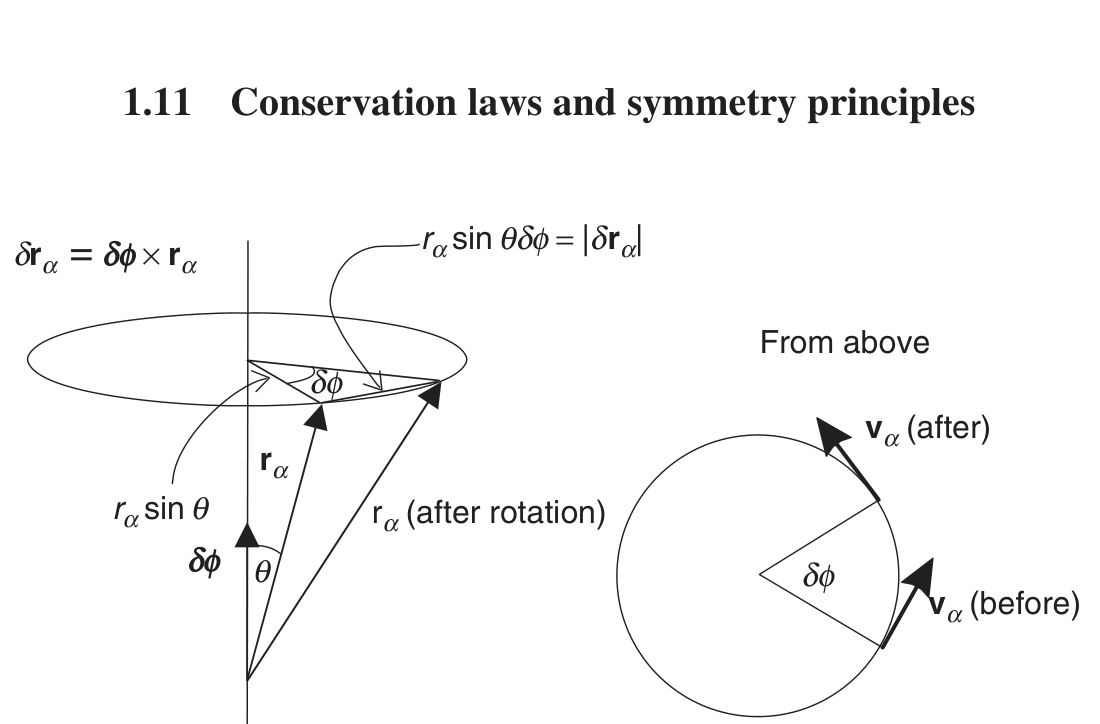
\includegraphics[width=0.55\linewidth]{Figure/fig_1_10.png}
\caption{图 1.10}
\end{figure}

系统的转动使每个质点的位置改变 $\delta\mathbf{r}_\alpha$，每个质点的速度改变 $\delta\mathbf{v}_\alpha$。

我们现在以更高级的方式处理这个问题，证明角动量守恒是空间各向同性的结果。

\begin{proof}[证明]
考虑一个绕某个轴转过虚角度 $\delta\phi$ 的力学系统。设 $\delta\bm{\phi}$ 是沿转轴方向、大小为 $\delta\phi$ 的矢量。把坐标原点放在转轴上。由于转动，系统中的每个质点都位移某个距离 $\delta\mathbf{r}_\alpha$，如果质点具有速度 $\mathbf{v}_\alpha$，速度矢量的方向将改变 $\delta\mathbf{v}_\alpha$。

如果空间是各向同性的，转动对拉格朗日量没有影响，所以 $\delta L = 0$，即
\begin{equation}\label{eq:1.dL2}
0 = \delta L = \sum_{\alpha}\left(\frac{\partial L}{\partial \mathbf{r}_\alpha}\cdot\delta\mathbf{r}_\alpha + \frac{\partial L}{\partial \mathbf{v}_\alpha}\cdot\delta\mathbf{v}_\alpha\right).
\end{equation}
（注意，在这种情况下，质点的速度不是常数。）

我们再次用拉格朗日方程把 $\dfrac{\partial L}{\partial \mathbf{r}_\alpha}$ 替换为 $\dfrac{d}{dt}\dfrac{\partial L}{\partial \mathbf{v}_\alpha} = \dfrac{d\mathbf{p}_\alpha}{dt} = \dot{\mathbf{p}}_\alpha$，并写
\begin{equation}\label{eq:1.ang1}
\sum_{\alpha}\left(\dot{\mathbf{p}}_\alpha\cdot\delta\mathbf{r}_\alpha + \mathbf{p}_\alpha\cdot\delta\mathbf{v}_\alpha\right) = 0.
\end{equation}
从图中，$|\delta\mathbf{r}| = r\sin\theta\,\delta\phi$。但由于 $\delta\mathbf{r}$ 同时垂直于 $\mathbf{r}$ 和 $\delta\bm{\phi}$，我们可以写 $\delta\mathbf{r} = \delta\bm{\phi}\times\mathbf{r}$。类似地，$\delta\mathbf{v} = \delta\bm{\phi}\times\mathbf{v}$。因此，
\begin{equation}\label{eq:1.ang2}
\sum_{\alpha}\left(\dot{\mathbf{p}}_\alpha\cdot(\delta\bm{\phi}\times\mathbf{r}_\alpha) + \mathbf{p}_\alpha\cdot(\delta\bm{\phi}\times\mathbf{v}_\alpha)\right) = 0.
\end{equation}
交换点乘和叉乘的次序，我们得到
\begin{equation}\label{eq:1.ang3}
\sum_{\alpha}\delta\bm{\phi}\cdot\left(\mathbf{r}_\alpha\times\dot{\mathbf{p}}_\alpha + \dot{\mathbf{r}}_\alpha\times\mathbf{p}_\alpha\right) = \delta\bm{\phi}\cdot\sum_{\alpha}\frac{d}{dt}\left(\mathbf{r}_\alpha\times\mathbf{p}_\alpha\right) = 0.
\end{equation}
因此，由于 $\delta\bm{\phi} \neq 0$，
\begin{equation}\label{eq:1.ang4}
\sum_{\alpha}\frac{d}{dt}(\mathbf{r}_\alpha\times\mathbf{p}_\alpha) = \frac{d}{dt}\sum_{\alpha}\mathbf{r}_\alpha\times\mathbf{p}_\alpha = \frac{d\mathbf{L}}{dt} = 0,
\end{equation}
其中 $\mathbf{L}$ 是总角动量。也就是说，空间各向同性导致角动量守恒。（注意不要把总矢量角动量 $\mathbf{L}$ 与拉格朗日量 $L$ 混淆。）
\end{proof}

\begin{example}[用初等力学证明角动量守恒]
用初等力学方法证明：如果没有净外力矩作用在系统上，质点系统的角动量就是常数。注意你必须援引强形式的牛顿第三定律。
\end{example}

\parahead{能量守恒与功函数}
考虑单个质点的动能。在初级物理中，我们学过功--能定理，它表明：外力对质点所做的净功，将导致质点动能的等量增加。按定义，功为
\begin{equation}\label{eq:1.W}
W = \int \mathbf{F}\cdot d\mathbf{s}.
\end{equation}
因此，受力 $\mathbf{F}$ 作用的质点从点 1 到点 2 的动能增加为
\begin{equation}\label{eq:1.W12}
T_2 - T_1 = \int_1^2 \mathbf{F}\cdot d\mathbf{s}.
\end{equation}
如果力是保守的，量 $\mathbf{F}\cdot d\mathbf{s}$ 就是一个标量量的微分，这个标量量记为 $U$，称为"功函数"。在现代术语中，功函数的概念已被势能（$V$）所取代，势能定义为功函数的负值：
\begin{equation}\label{eq:1.VU}
V = -U.
\end{equation}
这意味着，如果力是保守的，它可以用一个标量函数的梯度来表示，于是
\begin{equation}\label{eq:1.Fgrad}
\mathbf{F} = -\nabla V.
\end{equation}
那么功--能定理给出
\begin{equation*}
T_2 - T_1 = \int_1^2 -\nabla V\cdot d\mathbf{s}.
\end{equation*}
但 $\nabla V\cdot d\mathbf{s} = dV$，所以
\begin{equation*}
T_2 - T_1 = -(V_2 - V_1),
\end{equation*}
或
\begin{equation}\label{eq:1.Econs}
T_2 + V_2 = T_1 + V_1.
\end{equation}
这个方程表达机械能守恒；它表明，在保守力作用下，系统从一种位形到另一种位形的过程中，有一个量保持不变。这个量当然就是总机械能 $E = T + V$。

力是保守的条件是：它等于某个标量函数的负梯度。这等价于要求力的旋度为零，即 $\nabla\times\mathbf{F} = 0$。

以上关于能量守恒的讨论相当初等。我们现在从高级的角度考察能量，并证明能量守恒来自时间的均匀性。

\begin{proof}[证明]
一般来说，拉格朗日量 $L = L(q, \dot{q}, t)$ 对时间的导数为
\begin{equation}\label{eq:1.dLdt}
\frac{dL}{dt} = \sum_i\frac{\partial L}{\partial q_i}\frac{dq_i}{dt} + \sum_i\frac{\partial L}{\partial \dot{q}_i}\frac{d\dot{q}_i}{dt} + \frac{\partial L}{\partial t}.
\end{equation}
由拉格朗日方程，$\dfrac{\partial L}{\partial q_i} = \dfrac{d}{dt}\dfrac{\partial L}{\partial \dot{q}_i}$，所以
\begin{equation}\label{eq:1.dLdt2}
\frac{dL}{dt} = \sum_i\left[\dot{q}_i\frac{d}{dt}\frac{\partial L}{\partial \dot{q}_i} + \frac{\partial L}{\partial \dot{q}_i}\frac{d\dot{q}_i}{dt}\right] + \frac{\partial L}{\partial t}.
\end{equation}
但注意
\begin{equation}\label{eq:1.dsum}
\frac{d}{dt}\sum_i\dot{q}_i\frac{\partial L}{\partial \dot{q}_i} = \sum_i\left(\dot{q}_i\frac{d}{dt}\frac{\partial L}{\partial \dot{q}_i} + \frac{d\dot{q}_i}{dt}\frac{\partial L}{\partial \dot{q}_i}\right),
\end{equation}
所以前面方程中的求和可以用 $\dfrac{d}{dt}\sum_i\dot{q}_i\dfrac{\partial L}{\partial \dot{q}_i}$ 代替，
\begin{equation}\label{eq:1.dLdt3}
\frac{dL}{dt} = \frac{d}{dt}\sum_i\dot{q}_i\frac{\partial L}{\partial \dot{q}_i} + \frac{\partial L}{\partial t},
\end{equation}
或
\begin{equation}\label{eq:1.dLdt4}
\frac{\partial L}{\partial t} = \frac{d}{dt}\left(L - \sum_i\dot{q}_i\frac{\partial L}{\partial \dot{q}_i}\right).
\end{equation}
我们现在引入一个新量，称为\textbf{能量函数} $h$，定义为
\begin{equation}\label{eq:1.h}
h = h(q, \dot{q}, t) = \sum_i\dot{q}_i\frac{\partial L}{\partial \dot{q}_i} - L,
\end{equation}
所以
\begin{equation}\label{eq:1.dh}
\frac{\partial L}{\partial t} = -\frac{dh}{dt}.
\end{equation}
注意 $h$ 依赖于广义位置和广义速度。

让我们假定时间均匀性，使得时间不显式出现在拉格朗日量中。于是 $\dfrac{\partial L}{\partial t} = 0$，从而
\begin{equation}\label{eq:1.hcons}
\frac{d}{dt}\left(L - \sum_i\dot{q}_i\frac{\partial L}{\partial \dot{q}_i}\right) = -\frac{dh}{dt} = 0.
\end{equation}
也就是说，能量函数是常数。但这是否意味着能量（$E = T + V$）是常数？为了回答这个问题，我们注意到动能具有一般形式
\begin{equation}\label{eq:1.TTT}
T = T_0 + T_1 + T_2,
\end{equation}
其中 $T_0$ 不依赖于速度，$T_1$ 是速度的一次齐次函数，$T_2$ 是速度的二次齐次函数。\footnote{这可以从笛卡尔坐标中的动能出发，利用变换方程 $x = x(q_1, q_2, \ldots, q_n, t)$ 以及 $\dot{x}_i = \sum_j\frac{\partial x}{\partial q_j}\dot{q}_j + \frac{\partial x}{\partial t}$ 来证明。参见章末习题 1.7。}（在笛卡尔坐标中，$T_0$ 和 $T_1$ 都为零，$T_2$ 不仅对速度是二次的，而且实际上是速度的二次型，即它包含 $\dot{x}^2$ 而不包含 $\dot{x}\dot{y}$。）

回忆函数 $f(x_1, \ldots, x_n)$ 若满足
\begin{equation}\label{eq:1.hom}
f(\alpha x_1, \alpha x_2, \ldots, \alpha x_n) = \alpha^k f(x_1, \ldots, x_n),
\end{equation}
则称为 $k$ 次齐次函数。欧拉关于齐次函数的定理指出，若 $f$ 是 $k$ 次齐次的，则
\begin{equation}\label{eq:1.euler}
\sum_i x_i\frac{\partial f}{\partial x_i} = kf.
\end{equation}
由于动能具有 $T_0 + T_1 + T_2$ 的一般形式，拉格朗日量也具有这种形式：$L = L_0 + L_1 + L_2$。于是由欧拉定理，
\begin{equation*}
\sum_i\dot{q}_i\frac{\partial L_0}{\partial \dot{q}_i} = 0,
\end{equation*}
\begin{equation*}
\sum_i\dot{q}_i\frac{\partial L_1}{\partial \dot{q}_i} = L_1,
\end{equation*}
\begin{equation*}
\sum_i\dot{q}_i\frac{\partial L_2}{\partial \dot{q}_i} = 2L_2.
\end{equation*}
因此，
\begin{equation}\label{eq:1.L12}
\sum_i\dot{q}_i\frac{\partial L}{\partial \dot{q}_i} = \sum_i\dot{q}_i\frac{\partial (L_0 + L_1 + L_2)}{\partial \dot{q}_i} = L_1 + 2L_2,
\end{equation}
以及
\begin{equation}\label{eq:1.L20}
\sum_i\dot{q}_i\frac{\partial L}{\partial \dot{q}_i} - L = (L_1 + 2L_2) - (L_0 + L_1 + L_2) = L_2 - L_0.
\end{equation}
如果变换方程不显含 $t$，则 $T = T_2$，即 $T$ 是速度的二次齐次函数。如果 $V$ 不依赖于速度，则 $L_0 = -V$。于是
\begin{equation}\label{eq:1.hE}
h = T + V = E.
\end{equation}
只要这些条件得到满足，能量函数就等于总能量，总能量就守恒。
\end{proof}

如果我们把 $\dfrac{\partial L}{\partial \dot{q}_i}$ 替换为 $p_i$，能量函数就变换为哈密顿量，它是广义坐标和广义动量的函数：
\begin{equation}\label{eq:1.H}
H = H(q, p, t) = \sum_i\dot{q}_ip_i - L.
\end{equation}
能量函数和哈密顿量本质上是一回事，但它们是用不同的变量表示的，即 $h = h(q, \dot{q}, t)$ 和 $H = H(q, p, t)$。（$h$ 依赖于速度，而 $H$ 依赖于动量。）

\begin{example}
（a）证明 $\mathbf{F} = -y\hat{\mathbf{i}} + x\hat{\mathbf{j}}$ 不是保守的。（b）证明 $\mathbf{F} = y\hat{\mathbf{i}} + x\hat{\mathbf{j}}$ 是保守的。
\end{example}

\begin{example}
证明 $\mathbf{F} = 3x^2y\hat{\mathbf{i}} + (x^3 + 1)\hat{\mathbf{j}} + 9z^2\hat{\mathbf{k}}$ 是保守的。
\end{example}

\begin{example}
证明保守力的旋度为零。
\end{example}

\begin{example}
证明欧拉定理。（提示：对 $f(tx, ty, tz) = t^k f(x, y, z)$ 关于 $t$ 求导，然后令 $t = 1$。）
\end{example}

\begin{example}
证明 $z^2\ln(x/y)$ 是二次齐次的。
\end{example}

\begin{example}
证明
$$\sum_i\dot{q}_i\frac{\partial L_2}{\partial \dot{q}_i} = 2L_2.$$
\end{example}

\parahead{位力定理}
位力定理指出：对有界的保守系统（如绕恒星运行的行星），动能的平均值与势能的平均值成正比。（对行星/恒星系统，我们发现 $\langle T\rangle = -\frac{1}{2}\langle V\rangle$。）我们现在来证明这个定理。

\begin{proof}[证明]
在笛卡尔坐标中，动能是只依赖于速度的齐次二次函数，所以欧拉定理给出
\begin{equation}\label{eq:1.vir1}
\sum_{\alpha}\mathbf{v}_\alpha\cdot\frac{\partial T}{\partial \mathbf{v}_\alpha} = 2T.
\end{equation}
只要势能不依赖于速度，动量就可以表示为
\begin{equation*}
\mathbf{p}_\alpha = \frac{\partial T}{\partial \mathbf{v}_\alpha},
\end{equation*}
从而
\begin{equation}\label{eq:1.vir2}
2T = \sum_{\alpha}\mathbf{p}_\alpha\cdot\mathbf{v}_\alpha = \sum_{\alpha}\mathbf{p}_\alpha\cdot\frac{d\mathbf{r}_\alpha}{dt}.
\end{equation}
但
\begin{equation}\label{eq:1.vir3}
\frac{d}{dt}\sum_{\alpha}\mathbf{p}_\alpha\cdot\mathbf{r}_\alpha = \sum_{\alpha}\mathbf{p}_\alpha\cdot\frac{d\mathbf{r}_\alpha}{dt} + \sum_{\alpha}\frac{d\mathbf{p}_\alpha}{dt}\cdot\mathbf{r}_\alpha.
\end{equation}
因此
\begin{equation}\label{eq:1.vir4}
2T = \frac{d}{dt}\sum_{\alpha}\mathbf{p}_\alpha\cdot\mathbf{r}_\alpha - \sum_{\alpha}\frac{d\mathbf{p}_\alpha}{dt}\cdot\mathbf{r}_\alpha.
\end{equation}
现在由牛顿第二定律，对保守系统，
\begin{equation*}
\frac{d\mathbf{p}_\alpha}{dt} = \mathbf{F}_\alpha = -\frac{\partial V}{\partial \mathbf{r}_\alpha},
\end{equation*}
所以
\begin{equation}\label{eq:1.vir5}
2T = \frac{d}{dt}\sum_{\alpha}\mathbf{p}_\alpha\cdot\mathbf{r}_\alpha + \sum_{\alpha}\frac{\partial V}{\partial \mathbf{r}_\alpha}\cdot\mathbf{r}_\alpha.
\end{equation}
让我们求这个方程中所有项的平均值：
\begin{equation}\label{eq:1.vir6}
\langle 2T\rangle = \left\langle\frac{d}{dt}\sum_{\alpha}\mathbf{p}_\alpha\cdot\mathbf{r}_\alpha\right\rangle + \left\langle\sum_{\alpha}\mathbf{r}_\alpha\cdot\frac{\partial V}{\partial \mathbf{r}_\alpha}\right\rangle.
\end{equation}
回忆函数 $f(t)$ 的时间平均为
\begin{equation}\label{eq:1.avg}
\langle f(t)\rangle = \lim_{\tau\to\infty}\frac{1}{\tau}\int_0^{\tau} f(t)\,dt,
\end{equation}
所以
\begin{equation}\label{eq:1.vir7}
\left\langle\frac{d}{dt}\sum_{\alpha}\mathbf{p}_\alpha\cdot\mathbf{r}_\alpha\right\rangle = \lim_{\tau\to\infty}\frac{1}{\tau}\int_0^{\tau}\frac{d}{dt}\left(\sum_{\alpha}\mathbf{p}_\alpha\cdot\mathbf{r}_\alpha\right)dt = \lim_{\tau\to\infty}\frac{\sum_{\alpha}\mathbf{p}_\alpha\cdot\mathbf{r}_\alpha(\tau) - \sum_{\alpha}\mathbf{p}_\alpha\cdot\mathbf{r}_\alpha(0)}{\tau} = 0,
\end{equation}
其中我们假定 $\sum_{\alpha}\mathbf{p}_\alpha\cdot\mathbf{r}_\alpha$ 在所有时刻都保持有限。换句话说，我们假定运动是有界的，所以分子有限而分母趋于无穷大。

我们剩下
\begin{equation}\label{eq:1.vir8}
2\langle T\rangle = \left\langle\sum_{\alpha}\mathbf{r}_\alpha\cdot\frac{\partial V}{\partial \mathbf{r}_\alpha}\right\rangle.
\end{equation}
如果势能是位置的 $k$ 次齐次函数，那么由欧拉定理，右边为 $kV$，于是
\begin{equation}\label{eq:1.virial}
2\langle T\rangle = k\langle V\rangle.
\end{equation}
因此，例如，对引力场中质量为 $m$ 的质点，
\begin{equation}\label{eq:1.grav}
V = -\frac{GMm}{r},
\end{equation}
所以 $k = -1$，且
\begin{equation}\label{eq:1.virial.g}
2\langle T\rangle = -\langle V\rangle.
\end{equation}
\end{proof}
由于 $E = T + V$，我们看到 $\langle E\rangle = -\langle T\rangle$，这表明总能量为负，且平均动能的量值是平均势能量值的一半。

再举一个例子，考虑弹簧上的质量。势能为 $V = \frac{1}{2}Kx^2$，所以 $k = 2$，且 $2\langle T\rangle = 2\langle V\rangle$，即 $\langle T\rangle = \langle V\rangle$。
